\documentclass{article}
\usepackage{amsmath,amssymb,array}
\textheight 21cm
\textwidth 15cm
\usepackage{bm}
\usepackage{diagbox}
\usepackage{epsfig}
\usepackage{indentfirst}
\usepackage[colorlinks=true, linkcolor=red, citecolor=blue,CJKbookmarks=true]{hyperref}
\usepackage[top=1in, bottom=1in, left=1.25in, right=1.25in]{geometry}

\def\blue#1{{\textcolor{blue}{#1}}} % blue color
\def\red#1{{\textcolor{red}{#1}}} % red color
\newcommand{\bt}{\beta}
\newcommand{\ep}{\epsilon}
\newcommand{\f}{\frac}
\newcommand{\lt}{\left}
\newcommand{\n}{\nonumber}
\newcommand{\p}{\partial}
\newcommand{\rd}{{\rm d}}
\newcommand{\rt}{\right}
\newcommand{\ve}{\varepsilon}
\newcommand{\vp}{\varphi}
\newcommand{\arXg}[1]{\href{http://arxiv.org/abs/#1}{{\ttfamily arXiv:#1[gr-qc]}}}
\newcommand{\arXh}[1]{\href{http://arxiv.org/abs/#1}{{\ttfamily arXiv:#1[hep-th]}}}

\def\TeV{\mathrm{TeV}} % TeV
\def\GeV{\mathrm{GeV}} % GeV
\def\MeV{\mathrm{MeV}} % MeV
\def\keV{\mathrm{keV}} % keV
\def\kpc{\mathrm{kpc}} % keV
\def\eV{\mathrm{eV}} % keV
\def\um{\mu\mathrm{m}} % keV
\def\cm{\mathrm{cm}} % keV

\begin{document}



\begin{flushleft}
\textbf{Title:} Prospect for dark matter self-annihilation signatures from dwarf galaxies by LHAASO

\textbf{Manuscript ID:} DD12310/He

\textbf{Authors:} Dong-Ze He, Xiao-Jun Bi, Su-Jie Lin, Peng-Fei Yin and Xin Zhang
\end{flushleft}


We deeply appreciate the referees for providing the helpful and constructive comments on our manuscript.
Taking all these comments into account, we have submitted a revised version of our manuscript. Revised portion are marked in red in the attatched PDF file. The main responds to the comments and questions are listed as follows.
\vskip 1.5cm

\begin{center}
\textbf{\large Reply to the Comments of Referee A}
\end{center}

\vspace{3mm}

\begin{quote}
\emph{General comments: The authors estimate the sensitivity of the planned LHAASO air shower array to detect self-annihilating dark matter via gamma-ray emission from dwarf galaxies. The manuscript summarizes the methods and results: The authors consider a sample of 19 dwarf galaxies which are visible to the instrument. The instrument��s sensitivity and performance is combined with the expected flux to determine (using a likelihood-based approach) the sensitivity to a self-annihilation signal. Similar to previous studies, the uncertainty on the dark matter density in the dwarf galaxies is taking into account. The resulting sensitivity estimate to the self-annihilation rate is derived and presented.}

\emph{Originality and significance of the results: The approach used is very similar to previous works. The particular application to derive the sensitivity for LHAASO is to my knowledge new. Even though it is in principle a new result, it is not adding significantly to the general view on indirect searches for dark matter and it is not presenting a new methodology.}

\emph{Technical quality: The methods applied are (1) prediction of gamma-ray fluxes from self-annihilating Dark Matter (2) gamma-ray sensitivity of the instrument and (3) statistical analysis.}
%\vskip .5cm

\emph{The prediction (1) is based upon the standard calculation in this field (eq. 1,2,3), however the authors do not consider the absorption due to gamma-gamma pair-production in the cosmic-microwave background (most likely negligible below 100 TeV) and the absorption in the Galactic
photon field (probably negligible for most objects). The authors should demonstrate that these effects can be neglected.}
\end{quote}

\textbf{Reply:}
This question is quite relevant.
Most of this kind of works have not seriously discussed the absorption of the gamma-ray, but it is really an issue.
Our comments on this issue are given as follows.

First of all, the energy of current cosmic microwave background (CMB) photons is $E_{\rm CMB}\simeq6\times10^{-4}\,\eV$. The corresponding energy threshold of the injected gamma photons for the $e^+e^-$ pair production is
\begin{equation*}
  E_{\rm th} = \frac{2m_e^2c^4}{E_{\rm CMB}(1 - \rm{cos}\,\theta)} \gtrsim870\,\TeV.
\end{equation*}
Therefore, the photons of interest in this work would not be energetic enough to interact with the CMB.

Only the interstellar radiation field (ISRF) is able to absorb the target gamma-ray.
In Ref.~\cite{Mathis:1983fx}, Mathis et al. have shown that the infrared radiation in the Galaxy has a peak energy of $\sim100\,\um$ ($1.24\times10^{-2}\,\eV$) with the energy density $\sim0.05\,\eV/\cm^3$.
For the photons with energies above the threshold of these infrared radiations, we could roughly estimate the pair production cross section with the Thomson cross section $3\sigma_T/18\approx1.1087\times10^{-29}\,\rm{m}^2$~\cite{Gould:1967zzb}.
The survival probability of high energy photons after a length $d$ in the ISRF is
\begin{equation*}
  s \sim \exp(- n_{\rm IR} \times 3\sigma_T/18 \times d) = \exp\left(-\frac{1.379\times10^{-3}d}{\kpc}\right),
\end{equation*}
where $n_{\rm IR}$ is the number density of the infrared radiation, $d$ is the length of path that photons travel.
For a very conservative estimate, we adopt the most effective scattering angular $\theta$ and an overestimated cross section, and assume $d$ is the distance from the dSph to the Earth.
Even so, this survival probability is always larger than $90\%$ for the dSph with the distance less than $100\,\kpc$. Thus, we just assume the survival probability to be 100$\%$ and neglect the absorption effect in this work.

We have added these discussions at the end of Section III.A.

\vskip .5cm

\begin{quote}
\emph{The presentation of the calculation of the gamma-ray sensitivity of the instrument (2) is too brief
and leaves out important details. I would suggest to add these points: }

\emph{(a) the assumed observation time of one year: does the calculation include the visibility of the objects at widely different declination? Please list the effective time (which zenith angle range is considered) in Table I;}
\end{quote}

\begin{quote}
\emph{(b) the calculation of B and S (eqns. 4,5) seems to be neglecting energy dispersion/ energy resolution effects which are expected to be substantial at least for the WCDA;}
\end{quote}

\textbf{Reply:} We appreciate the referee for these two constructive suggestions. Our previous description for the calculation of $B$ and $S$ was indeed too brief. In the new version, we have re-expressed the eqs. (6) and (7) in a more detailed form,
\begin{equation*}
  B=\int^{E_{\rm max}}_{E_{\rm min}}\int_{\Delta\Omega}\int_0^T\zeta_{cr}\cdot\Phi_{p}(E)\cdot A_{\rm eff}^{p}(E,\theta_{\rm zen}(t))\cdot\varepsilon_{p}(E)dtd\Omega dE,
\end{equation*}
\begin{equation*}
  S=\epsilon_{\Delta\Omega}\int^{E_{\rm max}}_{E_{\rm min}}\int_0^T\Phi_{\gamma}(E)\cdot A_{\rm eff}^{\gamma}(E,\theta_{\rm zen}(t))\cdot\varepsilon_{\gamma}(E)dtdE,
\end{equation*}
where the relation between the event number $B$($S$) and the observation time $t$ is much clearer and the visibility of each dSph is obviously included.
In addition, as suggested by the referee, we have listed the ratio of effective observation time in the Table I as an estimation of the visibility.


\begin{quote}
\emph{(c) the energy ranges $E_{min}$ and $E_{max}$ for the integration for gamma-ray events (eq. 5) and for cosmic-ray events (eq. 4) are probably given in reconstructed energy --- however, the energy estimated for cosmic-ray nuclei induced air showers under-estimates their true energy. This leads to a wrong estimator of the background and therefore of the sensitivity;}
\end{quote}

\textbf{Reply:} This is a key point that we have considered but did not clearly demonstrate. In fact, we have chosen a much wider energy bin ($E_{\rm max}/E_{\rm min}=3$ for each bin) compared with the width of energy dispersion. When we count particles with the reconstructed energy, only a very small proportion of them falling around the boundary of the energy bin may be incorrectly counted. Therefore these statistic errors can be neglected in the practical calculation. We have added the comment on this issue in the third paragraph of Section III.B.

\begin{quote}\emph{(d) the angular resolution of LHAASO is not provided and should be included;}\end{quote}

\textbf{Reply:} The angular resolution for LHAASO-WCDA is varying from $2^\circ$ to $0.1^\circ$ with increased photon energy as shown in Fig. \ref{fig:angular-resolution} (this figure is not added in the paper as it is not a published result). The corresponding information has been added in the revised manuscript.
\begin{figure*}\centering
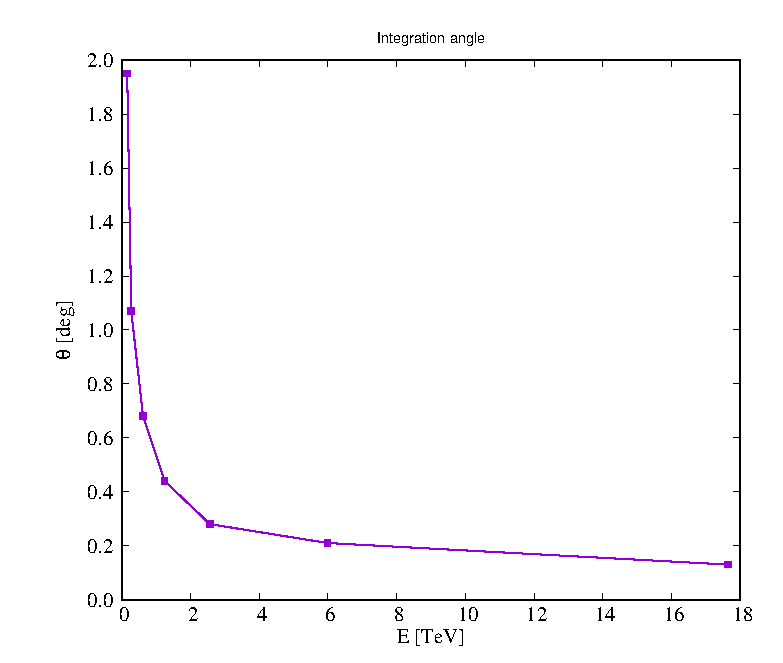
\includegraphics[width=0.60\textwidth]{theta.eps}
\caption{Energy dependent angular resolution for LHAASO-WCDA.}
\label{fig:angular-resolution}
\end{figure*}

\begin{quote}\emph{(d) gamma-hadron separation: the claimed gamma-hadron separation is in principle the central part of the study --- however, there is no reliable reference given (just a private communication). I am not convinced that the claimed gamma-hadron separation is realistic. Without a detailed study in a separate publication, it remains at least unclear to what extent the results presented in this paper are reliable;}\end{quote}

\textbf{Reply:} This is an essential point that we have not clarified in the previous version. In fact, the authors of Ref. \cite{Zha:2017vcs} have discussed the details of gamma-hadron separation for the LHAASO-WCDA detector. In this work, we adopted the survival ratios of  $\varepsilon_{p}= 0.278$ and $\varepsilon_{\gamma}= 40.13$ from a simulation, which are more conservative than the results in Ref. \cite{Zha:2017vcs}. We have discussed this issue and added Ref.~\cite{Zha:2017vcs} in the revised manuscript.

\begin{quote}\emph{(f) Furthermore, uncertainties in the collection area and efficiencies (and energy reconstruction) would need to be treated as additional nuisance parameters (similar to the uncertainty of J-factors) --- this is not the case. Please provide an argument why this is a negligible effect.}\end{quote}


\textbf{Reply:}
The referee has asked a quite critical question.
As shown in Fig.46 of Ref.~\cite{Bai:2019khm}, the statistical errors of the effective collection area are quite small (unlike the $J$-factor), therefore we did not take these uncertainties into account in the present calculation.
There may indeed exist some systematical errors in the effective area. However, up to now, no available result has been provided by the experimental group.
In fact, for the energy reconstruction, we have adopted wide energy bins to suppress the corresponding uncertainty mentioned above.
Therefore, the corresponding influence would be much smaller compared with that from the uncertainty of the $J$-factor. Thus, the uncertainties mentioned in this comment are not considered in the current circumstance.


\begin{quote}
\emph{Manuscript's presentation:}

\emph{Title: The title is not accurate --- the paper provides results on the expected sensitivity for gamma-ray emission from self-annihilating dark matter in dwarf galaxies. Currently, the title mentions ``dark matter signatures from dwarf galaxies" --- leaving open what kind of signatures are meant (e.g. anti-protons etc.).}
\end{quote}

\textbf{Reply:} We totally agree with the referee's suggestion. We have revised the title as ``Prospect for dark matter annihilation signatures from the gamma-ray observation of dwarf galaxies by LHAASO".

\begin{quote}
\emph{Abstract: The statement ``will observe with unprecedented sensitivity between 300 GeV .." is not correct. When looking at Fig. 1 it becomes immediately clear, that both MAGIC as well as HESS have a better sensitivity. Please remove this false claim. The $J$-factor is mentioned in the abstract without explaining what it is. It is better to replace it with ``uncertainty on the spatial Dark Matter distribution". The main result is the achievable constraint on the velocity-weighted cross-section --- it would be good to put this result in the context of the expected cross section in case of thermal dark matter generation which is a factor 10 to 100 smaller than the achievable sensitivity.}
\end{quote}

\textbf{Reply:} We have removed that false claim ``unprecedented sensitivity..." and rephrased the statement according to the comment. Besides, we have replaced ``$J$-factor" with ``uncertainties on the spatial DM distribution" in the Abstract part of the revised manuscript. We have also put our result in the context of the canonical thermal relic cross section as shown in the abstract of the revised manuscript according to the referee's comment.

\begin{quote}
\emph{Some general comments on the language:}

\emph{The use of language is in some cases not sufficiently accurate (e.g., [..] the propagation process of gamma-rays is not deflected [..] --- the process is not deflected, I hope) and includes some laboratory slang terms (e.g., mainstream DM [..]). }
\end{quote}

\textbf{Reply:} We are sorry for our inaccurate expressions. For these phrases, we have made corresponding modifications in the revised version according to the referee's comments.

\begin{quote}
\emph{The use of the term ``annihilation" should be more specific to be ``self-annihilation" (annihilation would include effects of co-annihilation --- also it is not clear whether Dirac or Majorana WIMPs are considered).}
\end{quote}

\textbf{Reply:} We have rephrased the sentences throughout the text at beginning of the second paragraph in the Page 2 of our revised manuscript to clarify this problem.

\begin{quote}
\emph{There are some factual problems as well, e.g., when stating that dwarf spheroidal galaxies are ``predicted by the CDM scenario" is somewhat giving a wrong impression for it is actually problematic to reconcile the small number of dwarf spheroidals with the larger number predicted in the framework of the CDM.}
\end{quote}

\textbf{Reply:} This phrase was modified according to the comment in the revised version.

\begin{quote}
\emph{Yet another example for missing accuracy in the introduction is at the bottom of page 2, where the progress in gamma-ray astronomy is limited to the past 20 years, while it is clear that the break-through discoveries were done already before that (e.g., with EGRET, Whipple etc.).}
\end{quote}

\textbf{Reply:} We totally agree with the referee. The first detection of TeV gamma rays was in thirty years ago, from the Crab Nebula with the Whipple experiment in 1989 \cite{Weekes:1989tc}. We have rephrased this inaccurate expression in the revised version.

\begin{quote}
\emph{On page 3, it is mentioned that HAWC takes advantage of the muon signal in air showers for gamma-hadron separation --- however, the gamma-hadron separation relies more on the lateral distribution of ionizing particles given that there are no shielded muon detectors present.}
\end{quote}

\textbf{Reply:} We have removed this inaccurate expression in the revised version.

\begin{quote}
\emph{Fig. 1: the difference between the sensitivity of WCDA and HAWC should be discussed somewhere. Given the larger surface area covered with the WCDA (a factor of 4.5), the sensitivity curves should differ by a factor of (4.5)$^{0.5}\sim$ 2.1. However, the difference is much larger (about a factor of 7 better). The angular resolution and gamma-hadron separation are probably similar in a realistic study.}
\end{quote}

\textbf{Reply:} We thank the referee for pointing out this critical issue.
The main reason for this difference is that the $\gamma/p$ discrimination adopted in this work is stricter than that of HAWC.
When the gamma efficiency $\varepsilon_\gamma$ is kept at $\sim50\%$, the survival ratio of the proton $\varepsilon_p$ (around $1\,\TeV$) is always larger than $1\%$ in the HAWC studies~\cite{Capistran:2015dua,Abeysekara:2017mjj}, whereas this value expected by WCDA is much smaller as shown in Ref.~\cite{Zha:2017vcs}.
In this work, we have adopted a relatively more conservative $\varepsilon_p \simeq 0.278\%$ for $\varepsilon_{\gamma} \simeq 40.13$, compared with those provided in Ref.~\cite{Zha:2017vcs}. In spite of this, the good $\gamma/p$ discrimination of WCDA still leads to an improvement with a factor of $\sim2$.

\begin{quote}
\emph{In summary, I recommend to reject the paper in its current form. The main reason for this is that the underlying sensitivity used is based upon a private communication and the crucial ingredients to this study remain undocumented. }
\end{quote}

\textbf{Reply:} Finally, we emphasize that the efficiencies for the gamma-hadron separation used in this work are more conservative than the public results from Ref. \cite{Zha:2017vcs}. We hope that the referee would find that our study is reliable and has reached the level for publication in Physcial Review D.

\vskip 1.5cm


\begin{center}
\textbf{\large Reply to the Comments of Referee B}
\end{center}


\begin{quote}
\emph{Page 6: In the last paragraph of III.A, $\theta_{max}$ remains undefined. Why is 0.5 deg used as upper bound for $\alpha_{int}$? An increasing number of background events is by itself not a problems as long as the signal-to-noise ratio still increases.}
\end{quote}

\textbf{Reply:}
This question is quite critical.
The previous description of this part is too brief and may lead to some misunderstanding.
We have reorganized this part in the revised manuscript to clarify the definition of $\theta_{\rm max}$ and the motivation of choosing a small $\alpha_{\rm int}$.
There are two sets of $J$-factors in Refs.~\cite{Geringer-Sameth:2014yza,Hutten:2016jko}, one set is derived with a constant integration angle $\alpha_{\rm int}=0.5^\circ$, and the other is derived with the integration angle which equals to the maximum angular radius $\alpha_{\rm int}=\theta_{\rm max}$.
The maximum angular radius $\theta_{\rm max}$ of each source is indicated by their outermost member star in the current observation.
The annihilation contribution of the gamma-ray signals, which is proportional to the DM density squared ($\rho^2$), would concentrate more around the center of the dSphs. Consequently, a smaller integration angle would always lead to a larger signal-to-background ratio in this work.
Therefore, in the Table.~I of the revised version, we choose the $J$-factor within a small integration angle as $\alpha_{\rm int}=\min\{\theta_{\rm max},0.5\}$.


\vskip 0.5cm
\begin{quote}
\emph{Caption Table I: Please explain what ``maximum angular radius $\theta_{max}$" is supposed to mean.}
\end{quote}

\textbf{Reply:} Generally speaking, $\theta_{\rm max}$ is taken to be ${\rm arcsin}(r_{\rm max}/D)$, where $r_{\rm max}$ is an estimate of distance from the center of dSph to the outermost member star and $D$ is the distance from Earth to the dSph. We have added the definition of $\theta_{\rm max}$ in the Caption of Table I.

\vskip 0.5cm
\begin{quote}
\emph{After Eq. (4): For CTA at low energies the electron CR background is a problem. I suppose this is no issue for the LHAASO energy range,
but it might be useful to briefly comment on that here.}
\end{quote}

\textbf{Reply:} This is a critical point. For the energies higher than $\sim300\,\GeV$, the CR electron background would be less than 30\%, and would rapidly decrease at higher energies.  We have added the comments about this issue in the revised version.

\vskip 0.5cm
\begin{quote}
\emph{The authors only use NFW profiles for estimating J-values. Please comment on the effect of using cored profiles instead.}
\end{quote}

\textbf{Reply:} We are sorry for our inaccurate description. In our work, we take the $J$-factors provided in Refs.~\cite{Geringer-Sameth:2014yza,Hutten:2016jko}. In Ref.~\cite{Geringer-Sameth:2014yza}, the $J$-factors are calculated by using the Zhao profile \cite{Hernquist:1990be,Zhao:1995cp}, which is parameterized as\
\begin{equation}
\rho(r)=\frac{\rho_s}{(r/r_s)^\gamma[1+(r/r_s)^\alpha]^{(\beta-\gamma)/\alpha}},
\end{equation}
where $\rho_s$, $r_s$, $\alpha$, $\beta$ and $\gamma$ are free parameters. For $(\alpha, \beta, \gamma)=(1,3,1)$, this profile becomes the standard NFW profile. However, this profile can also describe the cored halo for $\gamma\sim 0$. In principle, these free parameters in the density profile can be determined in the Jeans analysis of dSph kinematics. In principle, the free parameters in the profile can be extracted in the Jeans analysis of dSph kinematics, and then be used to derive the median value and credible interval of the $J$-factor. Another typical profile used in Ref.~\cite{Hutten:2016jko} is the Einasto profile~\cite{Graham:2005xx}, which is parameterized as
\begin{equation}
\rho(r)=\rho_{-2}\left\{ -\frac{2}{\alpha}\left[\left(\frac{r}{r_{-2}}\right)^\alpha-1\right] \right\},
\end{equation}
where $\rho_{-2}$, $r_s$, $r_{-2}$ and $\alpha$ are free parameters. As discussed in Ref.~\cite{Bonnivard:2014kza}, the results given by these two parameterisations are in very good agreement. We have added these descriptions in the revised manuscript.


\vskip 0.5cm
\begin{quote}
\emph{In Fig. 2, where does the structure in some of the upper limits come from (e.g. for $W^+W^-$, many of the lines show dips that extend over
factors of a few in $m_{DM}$). The fact that this does not affect all limits in the same way suggests that it cannot be an instrumental effect. What is causing it?}
\end{quote}

\textbf{Reply:} These structures should be attributed to the uncertainty of the $J$-factor. As mentioned in section III.B, those upper limits are derived from a series of simulated observations. In the observations, there would occasionally be some positive signals counts in some energy bins due to statistic fluctuations. Taking the uncertainty of the $J$-factor into account, the sensitivities at the energy bins with no pseudo signal count would be much stronger than those with some pseudo signal counts, which could finally lead to the random structures of the sensitivity curves varying with the $m_{\rm DM}$. It can be clearly seen that the dSphs with larger $J$-factor uncertainties always associate with stepper dips. When we consider plentiful mimic observations as seen in Fig. 3 of manuscript, these random dips would collectively contribute to the containment bands.

\vskip 0.5cm
\begin{quote}
\emph{In Fig. 3: The 68\% and 95\% containment regions look surprisingly wide (usually these bands only span factors of a few in the flux). Is this caused by the J-value uncertainties, or something else?}
\end{quote}

\textbf{Reply:} Yes, this is caused by the uncertainty of the $J$-factor. In Table I, the four dSphs marked with asterisks (Draco II, Pisces II, Triangulum II and Willman 1) with large $J$-factors have relatively large uncertainties. These uncertainties enlarge the containment regions.

\vskip 0.5cm
\begin{quote}
\emph{Last sentence of the conclusions: I'm all for searches for dark matter particles at all accessible energies. However, it is not clear to me if there are actually many theoretical (WIMP) models that could accommodate the large required cross-sections and DM masses necessary to produce actually a signal in LHAASO. Could you provide examples?}
\end{quote}

\textbf{Reply:} The referee has asked an enlightening question. If DM particles are dominantly produced via the freeze-out mechanism, it is difficult to detect the annihilation signal in LHAASO or other cherenkov detectors due to the small annihilation cross section required by the thermal relic density. However, if DM particles are produced non-thermally, they can still have a large annihilation cross section. There have been many non-thermal mechanisms proposed in the literature. For instance, the DM particles can be produced as the decay products of heavy particles, Q balls or cosmic strings (see e.g.~\cite{Moroi:1999zb,Fujii:2002kr,Jeannerot:1999yn} and references therein). We have added these discussions in the introduction section of the revised manuscript.

\vskip 0.5cm
\begin{quote}
\emph{Given that LHAASO has a very large field of few, I think that constraints derived from the non-observation of an excess associated with the entire Milky Way halo could be stronger than just the dSph constraints. It would be interesting to see estimates for that as well, although I understand if this is beyond the scope of the paper.}
\end{quote}

\textbf{Reply:} We totally agree with the referee. We will consider this enlightening point of view in the forthcoming work.

\vspace{2em}
\vskip .5cm

In summary, we are very grateful for the valuable comments and suggestions of the referees, and have already carefully revised our manuscript. We hope that the above answers will convince the referees that our work has been significantly improved and our revised manuscript is now suitable for publication in Physical Review D.

\bibliographystyle{unsrt}
\bibliography{reference}


\end{document}
